\documentclass{article}

\usepackage{fancyhdr}
\usepackage{extramarks}
\usepackage{amsmath}
\usepackage{amsthm}
\usepackage{amsfonts}
\usepackage{tikz}
\usepackage[plain]{algorithm}
\usepackage{algpseudocode}
\usepackage{enumerate}
\usepackage{tikz}
\usepackage{xifthen}
\usepackage{xparse}
\usepackage{amsmath, amssymb}
\usepackage{lipsum}
\usetikzlibrary{automata,positioning}

%
% Basic Document Settings
%  

\topmargin=-0.45in
\evensidemargin=0in
\oddsidemargin=0in
\textwidth=6.5in
\textheight=9.0in
\headsep=0.25in

\linespread{1.1}

\pagestyle{fancy}
\lhead{\hmwkAuthorName}
\chead{\hmwkClass : \hmwkTitle}
\rhead{\firstxmark}
\lfoot{\lastxmark}
\cfoot{\thepage}

\renewcommand\headrulewidth{0.4pt}
\renewcommand\footrulewidth{0.4pt}

\setlength\parindent{0pt}

%
% Create Problem Sections
%

\newcommand{\enterProblemHeader}[1]{
    \nobreak\extramarks{}{Problem \arabic{#1} continued on next page\ldots}\nobreak{}
    \nobreak\extramarks{Problem \arabic{#1} (continued)}{Problem \arabic{#1} continued on next page\ldots}\nobreak{}
}

\newcommand{\exitProblemHeader}[1]{
    \nobreak\extramarks{Problem \arabic{#1} (continued)}{Problem \arabic{#1} continued on next page\ldots}\nobreak{}
    \stepcounter{#1}
    \nobreak\extramarks{Problem \arabic{#1}}{}\nobreak{}
}

\newcommand*\circled[1]{\tikz[baseline=(char.base)]{
		\node[shape=circle,draw,inner sep=2pt] (char) {#1};}}


\setcounter{secnumdepth}{0}
\newcounter{partCounter}
\newcounter{homeworkProblemCounter}
\setcounter{homeworkProblemCounter}{1}
\nobreak\extramarks{Problem \arabic{homeworkProblemCounter}}{}\nobreak{}

%
% Homework Problem Environment
%
% This environment takes an optional argument. When given, it will adjust the
% problem counter. This is useful for when the problems given for your
% assignment aren't sequential. See the last 3 problems of this template for an
% example.
%

\newenvironment{homeworkProblem}[1][-1]{
    \ifnum#1>0
        \setcounter{homeworkProblemCounter}{#1}
    \fi
    \section{Problem \arabic{homeworkProblemCounter}}
    \setcounter{partCounter}{1}
    \enterProblemHeader{homeworkProblemCounter}
}{
    \exitProblemHeader{homeworkProblemCounter}
}

%
% Homework Details
%   - Title
%   - Class
%   - Due date
%   - Name
%   - Student ID

\newcommand{\hmwkTitle}{Homework\ \#02}
\newcommand{\hmwkClass}{Probability \& Statistics for EECS}
\newcommand{\hmwkDueDate}{Feb 26, 2023}
\newcommand{\hmwkAuthorName}{Wang Yunfei}
\newcommand{\hmwkAuthorID}{2021533135}


%
% Title Page
%

\title{
    \vspace{2in}
    \textmd{\textbf{\hmwkClass:\\  \hmwkTitle}}\\
    \normalsize\vspace{0.1in}\small{Due\ on\ \hmwkDueDate\ at 23:59}\\
	\vspace{4in}
}

\author{
	Name: \textbf{\hmwkAuthorName} \\
	Student ID: \hmwkAuthorID}
\date{}

\renewcommand{\part}[1]{\textbf{\large Part \Alph{partCounter}}\stepcounter{partCounter}\\}

%
% Various Helper Commands
%

% Useful for algorithms
\newcommand{\alg}[1]{\textsc{\bfseries \footnotesize #1}}
% For derivatives
\newcommand{\deriv}[1]{\frac{\mathrm{d}}{\mathrm{d}x} (#1)}
% For partial derivatives
\newcommand{\pderiv}[2]{\frac{\partial}{\partial #1} (#2)}
% Integral dx
\newcommand{\dx}{\mathrm{d}x}
% Alias for the Solution section header
\newcommand{\solution}{\textbf{\large Solution}}
% Probability commands: Expectation, Variance, Covariance, Bias
\newcommand{\E}{\mathrm{E}}
\newcommand{\Var}{\mathrm{Var}}
\newcommand{\Cov}{\mathrm{Cov}}
\newcommand{\Bias}{\mathrm{Bias}}

\begin{document}

\maketitle

\pagebreak

\begin{homeworkProblem}[1]
\solution
\section{(a)}
    From the question, we can easily get this is an ordered with replacement sample, so the answer is $n^n$.

\section{(b)}
    From the question, we can get similarly that this is an unordered with replacement sample. It can be represented as $(c_1,c_2,\cdots,c_n)$, 
    in which $c_i$ is the times of choosing $a_i$, and $1<=i<=n$. So we can have $c_1+c_2+\cdots+c_n=n$, and $c_i>=0$. Finally, we can get the answer:\\
    $\binom{n+n-1}{n-1}=\binom{2n-1}{n-1}$.

\section{(c)}
\subsection{(01)}
    From what we have defined in (b) and the multinomial theorem, we can transfer the answer into another way, that is $\frac{n!}{n_1!n_2!\cdots n_n!}$
    for every unordered bootstrap sample. And then divide by $n^n$ to get the corresponding probability which is equal to $\frac{n!}{n^nn_1!n_2!\cdots n_n!}$
    So we can define P(an unordered bootstrap sample)=$\frac{n!}{n^nn_1!n_2!\cdots n_n!}$. So we can prove what we want, because $n^n$ and $n!$ are all constant number, 
    thus different unordered bootstrap samples may be not equally likely due to $n_1!n_2!\cdots n_n!$ is not equal.
\subsection{(02)}
    For $b_1$ which is as likely as possible, so we need to minimum $n_1!n_2!\cdots n_n!$, and then let $n_1=n_2=\cdots=n_n=1$. Finally we can get it.\\
    For $b_2$ which is as unlikely as possible, so we need to maximum $n_1!n_2!\cdots n_n!$, and then we can let one element which is one of the elements in the range of 1 to n be equal to n, and let others be equal to 0.
    And then we can get what we want.
\subsection{(03)}
    So $p_1=P(b_1)=\frac{n!}{n^n}$ and $p_2=P(b_2)=\frac{n!}{n^nn!}$. Finally we can get $p_1/p_2=n!$.
\subsection{(04)}   
    For $b_1$, we just have one case, that is $(1,1,\cdots,1)$ and there are $1*n(n-1)\cdots 1=n!$ ways. But for $b_2$, we have n cases, \\
    that is $(n,0,\cdots,0),(0,n,\cdots,0)\cdots(0,0,\cdots,n)$ and it is just $1*n=n$ ways. Therefore, the ratio of the probability of getting an unordered
    bootstrap sample whose probability is $p_1$ to the probability of getting an unordered sample whose probability is $p_2$ is $n!/n=(n-1)!$.

\end{homeworkProblem}
\newpage
\begin{homeworkProblem}[2]

\begin{enumerate}
    \item
    Assume that event S: collect all 108 types of coupons. $P(S)$ represents the probability of collecting all 108 types of coupons.\\
    And for this question, the total number of cases is $108^n$, and the nature of the question is second class Stirling number, in which
    substitute n unequal purchases into the set corresponding to the 108 different coupons. Finally it can be represented as $S(n,108)*108!$.
    So $P(S)=\frac{S(n,108)*108!}{108^n}=\frac{\frac{1}{108!}*108!\sum_{k=0}^{108}(-1)^k \binom{108}{k}(108-k)^n}{108^n}$\\
    Therefore, the final result is $\frac{\sum_{k=0}^{108}(-1)^k \binom{108}{k}(108-k)^n}{108^n}$. 
    And then we can calculate it by python to get the final answer. The figure is as follow:\\
    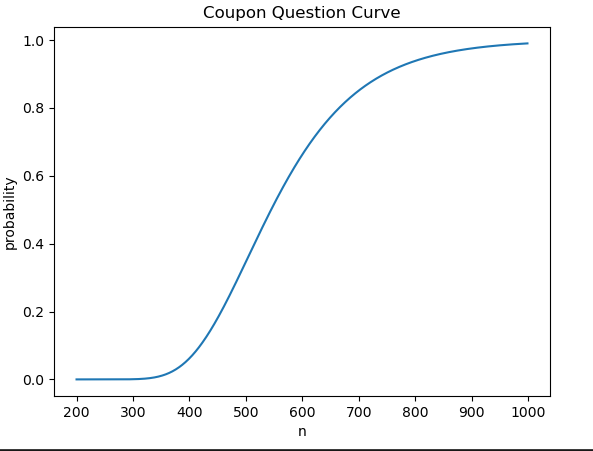
\includegraphics[scale=0.4]{QQ图片20230226152843}\\
    And the minimum number of n which makes the probability no less than 95 percents is 823.

\end{enumerate}

\end{homeworkProblem}

\begin{homeworkProblem}[3]
\solution
\begin{enumerate}
    \item The answer in this problem is obvious to get it. The total number of possible cases is $\binom{100}{4}=3921225$.
    And for cases where we do not pick a defective product, theirs number is equal to $\binom{95}{4}=3183545$, because there are five defectives.
    So the probability that the batch is accepted if it contains five defectives is equal to $\binom{95}{4}/\binom{100}{4}=3183545/3921225=0.8119$.

\end{enumerate}
\end{homeworkProblem}
\begin{homeworkProblem}[4]
\solution
    \begin{enumerate}
        \item 
        First assume event S as the situation that we get the gold, we can have:\\
        So the probability of get the gold in case a is $P(S|a)=1$\\
        The probability of get the gold in case b is $P(S|b)=0$\\
        The probability of get the gold in case c is $P(S|c)=1/2$\\
        Moreover $P(a)=P(b)=P(c)$.
        And then we can use the total probability theorem to get the $P(S)$, 
        that is $P(S)=P(S|a)*P(a)+P(S|b)*P(b)+P(S|c)*P(c)=1/2$. 
        At the same time, the probability of the next coin drawn from the same box also
        being a gold coin is equal to $P(S|a)*P(a)/P(S)=2/3$.
    \end{enumerate}
\end{homeworkProblem}
\begin{homeworkProblem}[5]
\solution
    \begin{enumerate}[(a)]
        \item
        The answer is $p_w^2(2-p_w)$, because there are two cases, Mirana wins in both games or Mirana wins one game and loses one game, and finally wins during sudden death.
    \end{enumerate}
    \begin{enumerate}[(b)]
        \item
        The answer is $p_d^2p_w$, because when she plays timid, it is only possible to win at sudden death after two draws.
    \end{enumerate}
    \begin{enumerate}[(c)]
        \item
        Assume event a as playing bold, and event b as playing timid. $P(a)=P(b)=1/2$, if there are not other requests.\\
        If the score is tied or behind $P(a') = 1$, and if the score leads $P(b')=1$.\\
        Therefore, we have five cases which are need to calculate:\\
        (1)First, Mirana plays bold in game 1 and wins, and then plays timid in game 2 and draws. $P(1)=P(a')*p_d*p_w=p_dp_w$.\\
        (2)Second, Mirana plays bold in game 1 and wins, but plays timid in game two and loses, and during sudden death plays bold and wins. 
        $P(2)=P(a')*p_w*(1-p_d)*p_w=p_w^2-p_dp_w^2$.\\
        (3)Third, Mirana plays bold in game1 but lose, and then plays bold in game 2 and wins, and during sudden death plays bold and wins.
        $P(3)=P(a')*(1-p_w)*p_w*p_w=p_w^2-p_w^3$.\\
        %%(4)Fourth, Mirana plays timid in game 1 and draws, and then plays bold in game 2 and wins. $P(4)=P(b)*p_d*p_w$.\\
        %%(5)Fifth, Mirana plays timid in game 1 and loses, and then plays bold in game 2 and wins, and during sudden death plays bold and wins.
        %%$P(5)=P(b)*(1-p_d)*p_w*p_w$.\\
        Finally, $P(Mirana\ wins\ under\ the\ strategy\ in\ c)=P(1)+P(2)+P(3)=-p_w^3-p_dp_w^2+2p_w^2+p_dp_w$.
    \end{enumerate}
    \begin{enumerate}[(d)]
        \item From the question we have $P(Mirana\ wins\ under\ the\ strategy\ in\ c)>=0.5$.\\
         And then we can simplify the form, that is $p_d>=\frac{0.5+p_w^3-2p_w^2}{p_w-p_w^2}$.\\
         So what we need to do is to find whether there is a $p_d$ which is greater than 0 and less than 1 when $p_w$ is less than 0.5 and greater than 0.
         Then we have $0<\frac{0.5+p_w^3-2p_w^2}{p_w-p_w^2}<1$. Analyze it from the left side, we just have $0.5+p_w^3-2p_w^2>0$. \\
         Let $F(p_w)=0.5+p_w^3-2p_w^2$, and then $F'(p_w)=3p_w^2-4p_w=3(p_w-\frac{2}{3})^2-\frac{4}{3}$ and because we have known $0<p_w<1/2$. \\
         And the zeros are 0 and 4/3, so $F'(p_w)<0$ in the given region. So $F(p_w)$ is monotonically decreasing and then let $p_w=0.5$, \\
         we can get the minimum value of $F(p_w)$. Therefore we have $F(0.5)=1/8>0$, which means we can have a satisfied $p_d$. \\
         At the same time, we can analyze it from the right side similarly, and get the same conclusion.\\
         Finally we prove that depending on the values of pw and pd, Mirana may have a better than a 50-50 chance to win the match. \\
         Intuitively, let $p_d=1$ and $p_w=0.5$, then we can easily get $P(Mirana\ wins\ under\ the\ strategy\ in\ c)=5/8>0.5$, so we can get it.
       
  
    \end{enumerate}
\end{homeworkProblem}    
\end{document}
